\chapter{Máquinas de Turing}
\label{cha:MTs}

Estudamos até aqui modelos de computação de expressividade crescente.
Começamos com autômatos finitos, vimos que existem linguagens que não conseguimos reconhecer com esse tipo de autômatos.
Identificamos exatamente a classe de linguagens que esse tipo de modelo é capaz de reconhecer, a saber, as linguagens regulares.
Passamos então para os autômatos com pilha que são mais expressivos, reconhecem todas as liguagens regulares e mais algumas não-regulares.
Novamente encontramos limitações, linguagens que não são reconhecíveis por autômatos com pilha.

Neste capítulo estudaremos um modelo ainda mais expressivo, as Máquinas de Turing (MTs).
Temos dois grandes objetivos neste capítulo.
O primeiro é convencer que este é o modelo definitivo de computação, ou seja, que não existe modelo de computação mais expressivo que as Máquinas de Turing.
Esse resultado, que não é nem pode ser um teorema, é chamado de Tese de Church-Turing.
O argumento para esta tese serão três: provaremos que as MTs são mais expressivas que os autômatos com pilha, em seguida mostraremos uma serie de variantes das MTs e provaremos que todas são equivalentes (i.e. tem a mesma expressividade) e, por fim, provaremos que toda MT pode ser simulada por uma MT específica chamada de Máquina de Turing Universal.
O segundo objetivo deste capítulo é provar que, mesmo sendo o modelo de computação mais completo, as MTs possuem limitações. 
Ou seja, existem problemas computacionais que não podem ser resolvidos por MTs.


\section{Máquinas de Turing Determinísticas}
\label{sec:MTs}

Uma MT consiste de uma fita formada por células em sequência, potencialmente infinita em ambas as direções e uma cabeça que lê o conteúdo de cada célula e guarda o estado atual.
Uma função de transição indica, dado o estado atual e o símbolo sendo lido qual é a próxima operação: ir para esquerda ou ir para a direita e qual o novo símbolo na célula atual.

Formalmente temos que uma {\em Máquina de Turing Determinística}, ou simplesmente uma MT, é uma 7-upla $\langle Q, \Sigma, \Gamma, \delta, q_0, q_a, q_r \rangle$ em que:
\begin{itemize}
\item[] $Q$ é um conjunto finito de {\em estados},
\item[] $\Sigma$ é o {\em alfabeto da entrada},
\item[] $\Gamma$ é o {\em alfabeto da fita} e $\Sigma \cup \{\textvisiblespace\} \subseteq \Gamma$,
\item[] $\delta: Q \times \Gamma \to Q \times \Gamma \times \{E, D\}$ é a {\em função de transição},
\item[] $q_0 \in Q$ é o {\em estado inicial},
\item[] $q_a \in Q$ é o {\em estado de aceitação} e
\item[] $q_r \in Q$ é o {\em estado de rejeição}.  
\end{itemize}

A cada passo, a MT está e, uma certa {\em configuração}.
A configuração indica a sequência de símbolos antes da cabeça na fita e a sequência de símbolos depois da cabeça.
Uma configuração pode ser representada por uma string da seguinte forma:
\begin{displaymath}
  C = \omega_1 q \omega_2
\end{displaymath}

As strings $\omega_1 \in \Gamma^*$ e $\omega_2 \in \Gamma^*$ indicam as sequências antes e depois da cabeça.
O estado $q$ indica o estado atual e o primeiro símbolo de $\omega$ dois é o símbolo sendo lido.
Uma configuração em que $q = q_a$ é dita de {\em aceitação} e em que $q = q_r$ é de {\em rejeição}.
Configurações de aceitação ou de rejeição são ditas {\em configurações de parada}.
A {\em função de transição} define para cada configuração $C_i$ qual o próxima configuração $C_{i+1}$.


\begin{example}
  \begin{enumerate}
  \item $uaq_i bv \Rightarrow uq_j acv$ se $\delta(q_i,b) = \langle q_j, c, E\rangle$

    \begin{center}
  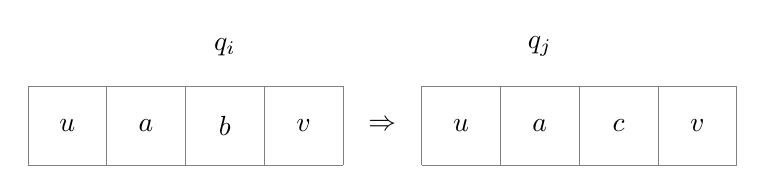
\begin{tikzpicture}
    \draw[help lines] (0,0) grid (4,1);
    \node at (0.5,0.5) {$u$};
    \node at (1.5,0.5) {$a$};
    \node at (2.5,0.5) {$b$};
    \node at (3.5,0.5) {$v$};
    \node at (2.5,1.5) {$q_i$};

    \node at (4.5,0.5) {$\Rightarrow$};

    \draw[help lines] (5,0) grid (9,1);
    \node at (5.5,0.5) {$u$};
    \node at (6.5,0.5) {$a$};
    \node at (7.5,0.5) {$c$};
    \node at (8.5,0.5) {$v$};
    \node at (6.5,1.5) {$q_j$};
  \end{tikzpicture}
\end{center}
    
\item $uaq_i bv \Rightarrow uacq_j v$ se $\delta(q_i,b) = \langle q_j, c, D\rangle$

      \begin{center}
  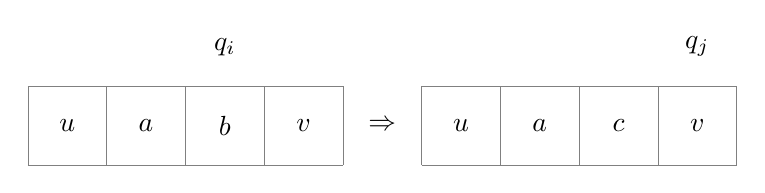
\begin{tikzpicture}
    \draw[help lines] (0,0) grid (4,1);
    \node at (0.5,0.5) {$u$};
    \node at (1.5,0.5) {$a$};
    \node at (2.5,0.5) {$b$};
    \node at (3.5,0.5) {$v$};
    \node at (2.5,1.5) {$q_i$};

    \node at (4.5,0.5) {$\Rightarrow$};

    \draw[help lines] (5,0) grid (9,1);
    \node at (5.5,0.5) {$u$};
    \node at (6.5,0.5) {$a$};
    \node at (7.5,0.5) {$c$};
    \node at (8.5,0.5) {$v$};
    \node at (8.5,1.5) {$q_j$};
  \end{tikzpicture}
\end{center}
  
\item $uaq_i b \Rightarrow uabq_j \textvisiblespace$ se $\delta(q_i,b) = \langle q_j, b, D\rangle$

      \begin{center}
  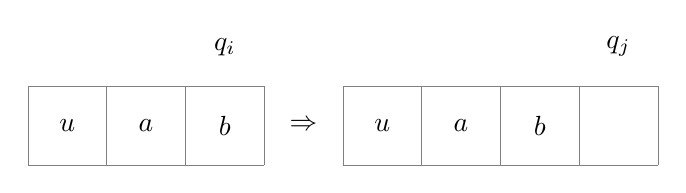
\begin{tikzpicture}
    \draw[help lines] (0,0) grid (3,1);
    \node at (0.5,0.5) {$u$};
    \node at (1.5,0.5) {$a$};
    \node at (2.5,0.5) {$b$};
    \node at (2.5,1.5) {$q_i$};

    \node at (3.5,0.5) {$\Rightarrow$};

    \draw[help lines] (4,0) grid (8,1);
    \node at (4.5,0.5) {$u$};
    \node at (5.5,0.5) {$a$};
    \node at (6.5,0.5) {$b$};
    \node at (7.5,1.5) {$q_j$};
  \end{tikzpicture}
\end{center}
  
\item $q_i uab \Rightarrow q_j \textvisiblespace uab$ se $\delta(q_i,u) = \langle q_j, u, E\rangle$

        \begin{center}
  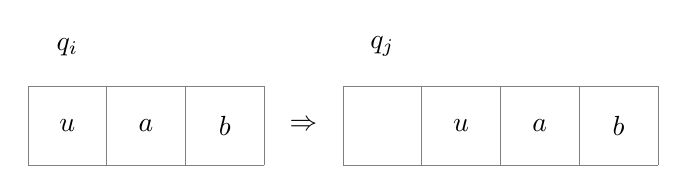
\begin{tikzpicture}
    \draw[help lines] (0,0) grid (3,1);
    \node at (0.5,0.5) {$u$};
    \node at (1.5,0.5) {$a$};
    \node at (2.5,0.5) {$b$};
    \node at (0.5,1.5) {$q_i$};

    \node at (3.5,0.5) {$\Rightarrow$};

    \draw[help lines] (4,0) grid (8,1);
    \node at (5.5,0.5) {$u$};
    \node at (6.5,0.5) {$a$};
    \node at (7.5,0.5) {$b$};
    \node at (4.5,1.5) {$q_j$};
  \end{tikzpicture}
\end{center}
  \end{enumerate}
\end{example}



Uma MT {\em aceita} uma string $\omega \in \Sigma^*$ se existe uma sequência de configurações $C_1, C_2, \dots, C_k$ em que:
\begin{enumerate}
\item $C_1 = q_0 \omega$ (configuração inicial),
\item $C_i \Rightarrow C_{i+1}$ para $i < k$ e
\item $C_k = \omega_1 q_a \omega_2$ (configuração de aceitação)
\end{enumerate}

Uma MT {\em rejeita} uma string $\omega \in \Sigma^*$ se existe uma sequência de configurações que satisfaz os dois primeiros itens e o seguinte:
\begin{enumerate}
\item[3'] $C_k = \omega_1 q_r \omega_2$ (configuração de rejeição) 
\end{enumerate}

Note que para rejeitar uma string não basta não aceitá-la.

Uma linguagem $A$ é {\em Turing-reconhecível} ou {\em recursivamente enumerável} (r.e.) se existe uma MT que aceita todas as strings de $A$.
Um linguagem $B$ é {\em Turing-decidível} ou {\em recursiva} se existe uma MT que aceita todas as strings em $B$ e rejeita todas as strings em $\bar{B}$.  


\begin{example}
  A linguagem $L(a^*b^*)$ é recursiva.

   \begin{tikzpicture}[node distance=2cm,auto,>=latex, every node/.style={sloped}]
    \tikzset{initial text={}}
    \node[circle, draw, initial] (q0) {};
    \node[circle, draw] (q1) at (2,0) {};
    \node[state] (qr) at (4,0) {$q_r$};
    \node[state] (qa) at (1,-2) {$q_a$};
    \path[->] (q0) edge[loop above] node {\tiny $a \rightarrow D$} (q0);
    \path[->] (q1) edge[loop above] node {\tiny $b \rightarrow D$} (q1);
    \path[->] (q0) edge node {\tiny $b \rightarrow D$} (q1);
    \path[->] (q1) edge node {\tiny $a \rightarrow E$} (qr);
    \path[->] (q0) edge node {\tiny $\textvisiblespace \rightarrow E$} (qa);
    \path[->] (q1) edge node {\tiny $\textvisiblespace \rightarrow E$} (qa);
  \end{tikzpicture}
  
\end{example}

\begin{example}
  A linguagem $\{a^nb^nc^n : n \geq 0 \}$ é recursiva\footnote{Para não poluir o diagrama omitimos as transições para $q_r$}.

  \begin{tikzpicture}[node distance=2cm,auto,>=latex, every node/.style={sloped}]
    \tikzset{initial text={}}
    \node[circle, draw, initial] (q0) {};
    \node[circle, draw] (q1) at (2,0) {};
    \node[circle, draw] (q2) at (4,0) {};
    \node[circle, draw] (q3) at (6,0) {};
    \node[circle, draw] (q4) at (8,0) {};
    \node[circle, draw] (q5) at (10,0) {};
    \node[circle, draw] (q6) at (12,0) {};
    \node[state] (qa) at (11,2) {$q_a$};
    \node[circle, draw] (q7) at (4,-2) {};
    \node[circle, draw] (q8) at (6,-2) {};
    \node[circle, draw] (q9) at (8,-2) {};
    \node[circle, draw] (q10) at (10,-2) {};
 %   \node[circle, draw] (q11) at (8,-1) {};

    \path[->] (q1) edge[loop above] node {\tiny $a \rightarrow D$} (q1);
    \path[->] (q2) edge[loop above] node {\tiny $\times \rightarrow D$} (q2);
    \path[->] (q3) edge[loop above] node {\tiny $b \rightarrow D$} (q3);
    \path[->] (q4) edge[loop above] node {\tiny $\times \rightarrow D$} (q4);
    \path[->] (q6) edge[loop below] node {\tiny $\times \rightarrow E$} (q6);
    \path[->] (q7) edge[loop below] node {\tiny $a \rightarrow E$} (q7);
    \path[->] (q8) edge[loop below] node {\tiny $\times \rightarrow E$} (q8);
    \path[->] (q9) edge[loop below] node {\tiny $b \rightarrow E$} (q9);
    \path[->] (q10) edge[loop below] node {\tiny $\times \rightarrow E$} (q10);
    
    \path[->] (q0) edge node {\tiny $a \rightarrow \times,D$} (q1);
    \path[->] (q1) edge node {\tiny $\times \rightarrow D$} (q2);
    \path[->] (q2) edge node {\tiny $b \rightarrow \times,D$} (q3);
    \path[->] (q3) edge node {\tiny $\times \rightarrow D$} (q4);
    \path[->] (q4) edge node {\tiny $c \rightarrow \times,D$} (q5);
    \path[->] (q5) edge node {\tiny $\textvisiblespace \rightarrow E$} (q6);
    \path[->] (q6) edge node {\tiny $\textvisiblespace \rightarrow E$} (qa);
    \path[->] (q5) edge node {\tiny $c \rightarrow E$} (q10);
    \path[->] (q10) edge node {\tiny $b \rightarrow E$} (q9);
    \path[->] (q9) edge node {\tiny $\times \rightarrow E$} (q8);
    \path[->] (q8) edge node {\tiny $a \rightarrow E$} (q7);
    \path[->] (q7) edge node {\tiny $\times \rightarrow D$} (q0);
%    \path[->] (q3) edge node {\tiny $c \rightarrow \times,D$} (q11);
%    \path[->] (q11) edge node {\tiny $\textvisiblespace \rightarrow E$} (q10);

    \path[->, bend left = 30] (q0) edge node {\tiny $\textvisiblespace \rightarrow D$} (qa);
    \path[->, bend right = 30] (q1) edge[below] node {\tiny $b \rightarrow \times,D$} (q3);
    \path[->, bend right = 30] (q3) edge[below] node {\tiny $c \rightarrow \times,D$} (q5);
  \end{tikzpicture}

\end{example}

\begin{example}
  \label{ex:eq}
A linguagem $\{\omega \# \omega : \omega \in \{a, b\}^*\}$ é recursiva.

  \begin{tikzpicture}[node distance=2cm,auto,>=latex, every node/.style={sloped}]
    \tikzset{initial text={}}
    \node[circle, draw, initial] (q0) {};
    \node[circle, draw] (q1) at (2,2) {};
    \node[circle, draw] (q2) at (4,2) {};
    \node[circle, draw] (q3) at (2,0) {};
    \node[circle, draw] (q4) at (4,0) {};
    \node[circle, draw] (q5) at (2,-2) {};
    \node[circle, draw] (q6) at (4,-2) {};
    \node[circle, draw] (q7) at (0,-2) {};
    \node[state] (qa) at (0,-4) {$q_a$};
    \node[state] (qr) at (7,0) {$q_r$};

    \path[->] (q0) edge[loop above] node {\tiny $\times \rightarrow D$} (q0);
    \path[->] (q1) edge[loop above] node {{\tiny $a \rightarrow D$},\\{\tiny $b \rightarrow D$}} (q1);
    \path[->] (q2) edge[loop above] node {\tiny $\times \rightarrow D$} (q2);
    \path[->] (q3) edge[loop above] node {{\tiny $a \rightarrow E$},\\{\tiny $b \rightarrow E$}} (q3);
    \path[->] (q4) edge[loop right] node {\tiny $\times \rightarrow E$} (q4);
    \path[->] (q5) edge[loop below] node {{\tiny $a \rightarrow D$},\\{\tiny $b \rightarrow D$}} (q5);
    \path[->] (q6) edge[loop below] node {\tiny $\times \rightarrow D$} (q6);
    \path[->] (q7) edge[loop left] node {\tiny $\times \rightarrow D$} (q7);

    \path[->] (q0) edge node {\tiny $b \rightarrow \times,D$} (q1);
    \path[->] (q1) edge node {\tiny $\# \rightarrow D$} (q2);
    \path[->] (q2) edge node {\tiny $b \rightarrow \times,E$} (q4);
    \path[->] (q2) edge node {{\tiny $\textvisiblespace \rightarrow D$},\\{\tiny $a \rightarrow D$}} (qr);
    \path[->] (q4) edge node {\tiny $\# \rightarrow E$} (q3);
    \path[->] (q3) edge node {\tiny $x \rightarrow D$} (q0);
    \path[->] (q0) edge node {\tiny $a \rightarrow \times,D$} (q5);
    \path[->] (q5) edge node {\tiny $\# \rightarrow D$} (q6);
    \path[->] (q6) edge node {\tiny $a \rightarrow \times,E$} (q4);
    \path[->] (q6) edge node {{\tiny $\textvisiblespace \rightarrow D$},\\{\tiny $b \rightarrow D$}} (qr);
    \path[->] (q0) edge node {\tiny $\# \rightarrow D$} (q7);
    \path[->] (q7) edge node {\tiny $\textvisiblespace \rightarrow D$} (qa);
  \end{tikzpicture}  

\end{example}

\begin{example}
  \label{ex:space}
  A Máquina de Turing a seguir tem o seguinte efeito:

  \begin{displaymath}
    \omega_1 q_i a \omega_2 \Rightarrow^* \omega_1 q_j \textvisiblespace a \omega_2
  \end{displaymath}

  \begin{tikzpicture}[node distance=2cm,auto,>=latex]
    \tikzset{initial text={}}
    \node[state] (qi) {$q_i$};
    \node[state] (qj) at (0,-2) {$q_j$};
    \node[circle, draw] (q1) at (2,0) {};
    \node[circle, draw] (q2) at (4,0) {};
    \node[circle, draw] (q3) at (6,2) {};
    \node[circle, draw] (q4) at (4,2) {};
    \node[circle, draw] (q5) at (4,-2) {};
    \node[circle, draw] (q6) at (6,-2) {};
    \node[circle, draw] (q7) at (2,-2) {};
    
    \path[->] (q1) edge[loop above, align=left] node {{\tiny $a \rightarrow D$}\\{\tiny $b \rightarrow D$}} (q1);

    \path[->] (qi) edge node {\tiny $a \rightarrow x,D$} (q1);
    \path[->] (q1) edge node {\tiny $\textvisiblespace \rightarrow E$} (q2);
    \path[->] (q2) edge node {\tiny $a \rightarrow D$} (q4);
    \path[->] (q4) edge node {\tiny $\textvisiblespace \rightarrow a,E$} (q3);
    \path[->] (q3) edge node {\tiny $a \rightarrow \textvisiblespace,E$} (q2);    
    \path[->] (q2) edge node {\tiny $b\rightarrow D$} (q5);
    \path[->] (q5) edge[below] node {\tiny $\textvisiblespace \rightarrow b,E$} (q6);
    \path[->] (q6) edge[right] node {\tiny $b \rightarrow \textvisiblespace,E$} (q2);
    \path[->] (q2) edge[left] node {\tiny $x \rightarrow \textvisiblespace,D$} (q7);
    \path[->] (q7) edge node {\tiny $\textvisiblespace \rightarrow a,E$} (qj);
  \end{tikzpicture}
  
\end{example}



\section{Máquinas de Turing Multifitas}
\label{sec:mt-fitas}

Uma variante das Máquinas de Turing são aquelas com múltiplas fitas.
Nesse caso, a cada passo temos $k$ símbolos sendos lidos e a função de transição indica o que fazer em cada uma das fitas dado o estado atual e os $k$ símbolos que estão sendo lidos.
Formalmente, como numa MT tradicional temas a seguinte tupla:

\begin{displaymath}
M = \langle Q, \Sigma, \Gamma, \delta, q_0, q_a, q_r \rangle
\end{displaymath}

Neste caso, porém, temos que:

\begin{displaymath}
\delta : Q \times \Gamma^k \to Q \times \Gamma^k \times \{E, D\}^k
\end{displaymath}

Ou seja, a função de transição leva um estado e $k$ símbolos em um novo estado, $k$ novos símbolos e $k$ direções.

\begin{example}
  \begin{displaymath}
    \delta(q_0, \langle a, b \rangle) = \langle q_1, \langle b,a \rangle, \langle D, D \rangle \rangle
  \end{displaymath}
  
  \begin{center}
    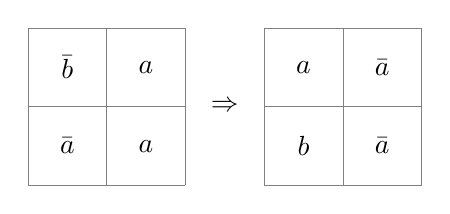
\begin{tikzpicture}
      \draw[help lines] (0,0) grid (2,2);
      \node at (0.5,0.5) {$\bar{a}$};
      \node at (1.5,0.5) {$a$};
      \node at (0.5,1.5) {$\bar{b}$};
      \node at (1.5,1.5) {$a$};

      \node at (2.5,1) {$\Rightarrow$};

      \draw[help lines] (3,0) grid (5,2);
      \node at (3.5,0.5) {$b$};
      \node at (4.5,0.5) {$\bar{a}$};
      \node at (3.5,1.5) {$a$};
      \node at (4.5,1.5) {$\bar{a}$};
    \end{tikzpicture}
  \end{center}
\end{example}

\begin{theorem}
  \label{theo:multifita}
  Para toda MT multifita existe uma MT simples equivalente.
\end{theorem}
\begin{proof}
  Faremos aqui apenas o esboço da prova.
  Simulamos as $k$ fitas em uma única fita com delimitadores indicados pelo símbolo $\#$.
  \begin{itemize}
  \item a entrada $a_1 \dots a_n$ será representada em uma única fita como $\# \bar{a_1} \dots a_n \# \textvisiblespace \# \dots \#$
  \item varre a entrada para verificar os símbolos sendo lidos
  \item varre novamente efetuando as transições em cada um dos trechos da fita
  \item se em algum ponto estivermos em $\#$ e a instrução for $D$ devemos abrir um espaço em branco antes de $\#$ (Exemplo \ref{ex:space}).
  \end{itemize}
\end{proof}

\begin{example}
  Considere o seguinte estado em uma MT multifita: 
  \begin{center}
    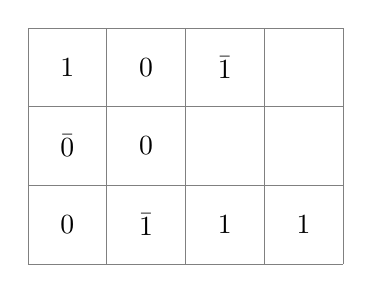
\begin{tikzpicture}
      \draw[help lines] (0,0) grid (4,3);
      \node at (0.5,0.5) {$0$};
      \node at (1.5,0.5) {$\bar{1}$};
      \node at (2.5,0.5) {$1$};
      \node at (3.5,0.5) {$1$};
      
      \node at (0.5,1.5) {$\bar{0}$};
      \node at (1.5,1.5) {$0$};

      \node at (0.5,2.5) {$1$};
      \node at (1.5,2.5) {$0$};
      \node at (2.5,2.5) {$\bar{1}$};
    \end{tikzpicture}
  \end{center}

  Ela seria representada em uma MT simples da seguinte forma:

  \begin{center}
    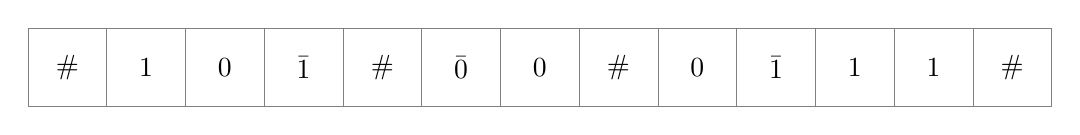
\begin{tikzpicture}
      \draw[help lines] (0,0) grid (13,1);

      \node at (0.5,0.5) {$\#$};
      \node at (1.5,0.5) {$1$};
      \node at (2.5,0.5) {$0$};
      \node at (3.5,0.5) {$\bar{1}$};

      \node at (4.5,0.5) {$\#$};
      \node at (5.5,0.5) {$\bar{0}$};
      \node at (6.5,0.5) {$0$};

      \node at (7.5,0.5) {$\#$};
      \node at (8.5,0.5) {$0$};
      \node at (9.5,0.5) {$\bar{1}$};
      \node at (10.5,0.5) {$1$};
      \node at (11.5,0.5) {$1$};
      \node at (12.5,0.5) {$\#$};
    \end{tikzpicture}
  \end{center}
  
\end{example}

\begin{theorem}
  Uma linguagem é recursiva se e somente se existem MTs que reconhecem $A$ e $\bar{A}$
\end{theorem}
\begin{proof}
  Se $A$ é recursivo então, por defineção existe uma MT $M$ que decide $A$ e, portanto, existe uma MT que reconhece $A$.

  Seja $M'$ uma MT igual a $M$ exceto que em $M'$ trocamos $q_a$ por $q_r$.
  A máquina $M'$ aceita tudo que $M$ rejeita e rejeita tudo que $M$ aceita.
  Portanto $M'$ reconhece $\bar{A}$.

  Agora sejam $M_1$ e $M_2$ MTs que reconhecem $A$ e $\bar{A}$ respectivamente.
  Construímos uma MT com duas fitas que simula $M_1$ e $M_2$ em paralelo.
  Ou seja, simula $M_1$ na primeira fita e $M_2$ na segunda.
  Essa MT deve aceitar $\omega$ se $M_1$ aceita $\omega$ e deve rejeitar $\omega$ se $M_2$ aceita $\omega$.
  Pelo Teorema \ref{theo:multifita} temos que existe uma MT simples equivalente a essa de fita dupla e esta MT decide $A$.
\end{proof}

\section{Máquinas de Acesso Aleatório (RAM)}
\label{sec:ram}

Vamos considerar agora uma máquina que a princípio parece bem diferente de uma MT, muito mais parecida com um computador moderno.
Uma {\em Máquina de Acesso Aleatório (RAM)} tem a capacidade de acessar um elemento qualquer em um único passo desde que ele esteja devidamente endereçado.

Em uma RAM temos um número de {\em registradores} capazes de armazenar e manipular {\em endereços} das células de memória.
Um {\em programa} em uma RAM é uma sequência de instruções que manipulam o conteúdo dos registradores e da memória.
O primeiro registrador tem uma função especial e é chamado {\em acumulador}.
Além disso, o programa mantém um contador $K$ que indica a instrução a ser executada.

\begin{center}
  \begin{tikzpicture}
    \draw[help lines] (0,1) grid (1,-3);
    
    \node at (0.5,0.5) {$K$};
    \node at (0.5,-0.5) {$R_0$};
    \node at (0.5,-1.5) {$\vdots$};
    \node at (0.5,-2.5) {$R_n$};
    
    \draw[help lines] (2,-1) grid (7,-2);
    
    \node at (2.5,-1.5) {$T[0]$};
    \node at (3.5,-1.5) {$T[1]$};
    \node at (4.5,-1.5) {$T[2]$};
    \node at (5.5,-1.5) {$T[3]$};
    \node at (6.5,-1.5) {$\dots$};
  \end{tikzpicture}
\end{center}

\begin{table}
  \label{tab:instrucoes}
  \centering
  \begin{tabular}{|ll|}
    \hline
    $read(j)$ & $R_0 \leftarrow T[R_j]$\\
    $write(j)$ & $T[R_j] \leftarrow R_0$\\
    $store(j)$ & $R_j \leftarrow R_0$\\
    $load(j)$ & $R_0 \leftarrow R_j$\\
    $load(=c)$ & $R_0 \leftarrow c$\\
    $add(j)$ & $R_0 \leftarrow R_0 + R_j$\\
    $add(=c)$ & $R_0 \leftarrow R_0 + c$\\
    $sub(j)$ & $R_0 \leftarrow R_0 - R_j$\\
    $sub(=c)$ & $R_0 \leftarrow R_0 - c$\\
    $half$ & $R_0 \leftarrow \lfloor R_0/2 \rfloor$\\
    $jump(s)$ & $K \leftarrow s$\\
    $jpos(s)$ & $R_0 > 0 \Rightarrow K \leftarrow s$\\
    $jzero(s)$ & $R_0 = 0 \Rightarrow K \leftarrow s$\\
    $halt$ & $K \leftarrow 0$\\
    \hline
  \end{tabular}
  \caption{Catálogo de instruções de uma RAM}
\end{table}

Uma {\em Máquina de Acesso Aleatório} (RAM) é um par $M = \langle k, \Pi \rangle$ em que $k > 0$ indica o número de registradores e $\Pi = \pi_0, \pi_1, \dots, \pi_n $ é uma sequência de instruções (programa) da Tabela \ref{tab:instrucoes} admitindo que $\pi_n = halt$. 

Formalmente um {\em configuração} de uma RAM é uma $k+2$-upla $\langle K, R_0, \dots, R_{k-1}, T\rangle$ em que:
\begin{enumerate}
\item $K \in \mathbb{Z}_p$ é o {\em contador de instruções}
\item uma {\em configuração de parada} é tal que $K = 0$
\item $R_j$ é o {\em valor do registrador} $j$
\item $T: \mathbb{N} \to \mathbb{N}$ leva um natural $i$ ({\em endereço}) em seu {\em conteúdo} $m$.
\end{enumerate}

Dizemos que a configuração $C = \langle K, R_0, \dots, R_{k-1}, T\rangle$ de uma RAM $M = \langle k, \Pi\rangle$ {\em produz em um passo} $C' = \langle K', R_0', \dots, R_{k-1}', T'\rangle$ (escrevemos $C \Rightarrow_M C'$) se $C'$ reflete o resultado da aplicação da instrução $\pi_K$ em $C$.
Se partindo de $C$ produzimos $C'$ em um número finito de passos, então escrevemos $C \Rightarrow^*_M C'$.

\begin{example}
  Considere a seguinte márquina $\langle \Pi, 4 \rangle$:
  \begin{multicols}{2}
    \begin{enumerate}
    \item $store(2)$
    \item $jzero(10)$
    \item $load(3)$
    \item $add(1)$
    \item $store(3)$
      \columnbreak
    \item $load(2)$
    \item $sub(=1)$
    \item $store(2)$
    \item $jump(1)$
    \item $load(3)$
    \item $halt$
    \end{enumerate}
  \end{multicols}
  
  Essa máquina começa com valores $n$ e $x$ nos registradores $0$ e $1$ e termina com $n \cdot x$ no acumulador.
  Ou seja, a maquina calcula a multiplicação.
%  Vamos simular com valore $2$ e $3$:

 % \begin{eqnarray*}
 %   1; 2, 3, 0, 0; \emptyset & \vdash & 1; 2, 3, 2, 0; \emptyset\\
 %                            & \vdash & 2; 2, 3, 2, 0; \emptyset\\
 %                            & \vdash & 3; 0, 3, 2, 0; \emptyset\\
 %                            & \vdash & 4; 3, 3, 2, 0; \emptyset\\
 %                            & \vdash & 5; 3, 3, 2, 3; \emptyset\\
 %                            & \vdash & 6; 2, 3, 2, 3; \emptyset\\
 %                            & \vdash & 7; 1, 3, 2, 3; \emptyset\\
 %                            & \vdash & 8; 1, 3, 1, 3; \emptyset\\
 %                            & \vdash & 1; 1, 3, 1, 3; \emptyset\\
 %                            & \vdash & 2; 3, 3, 1, 3; \emptyset\\
 %                            & \vdash & 3; 6, 3, 1, 3; \emptyset\\
 %                            & \vdash & 4; 6, 3, 1, 6; \emptyset\\
 %                            & \vdash & 5; 1, 3, 1, 6; \emptyset\\
 %                            & \vdash & 6; 0, 3, 1, 6; \emptyset\\
 %                            & \vdash & 7; 0, 3, 0, 6; \emptyset\\
 %                            & \vdash & 8; 0, 3, 0, 6; \emptyset\\
 %                            & \vdash & 1; 0, 3, 0, 6; \emptyset\\
 %                            & \vdash & 9; 6, 3, 0, 6; \emptyset\\
 %                            & \vdash & 10; 6, 3, 0, 6; \emptyset\\
 % \end{eqnarray*}

  Simulando com entrada $2$ e $3$ podemos conferir que:
\begin{displaymath}
\langle 1;2,3,0,0; \emptyset \rangle \Rightarrow_M^* \langle 11; 6,3,0,6; \emptyset\rangle
\end{displaymath}
  
Para faciliar a leitura e a escrita de programas podemos usar a abreviação $R_3 \leftarrow R_3 + R_1$ para a sequência comum de instruções $load(3)$, $add(1)$, $store(3)$ e $R_2 \leftarrow R_2 - 1$ para $load(2)$, $sub(=1)$, $store(2)$.
Além disso, podemos dar nomes como $x$, $y$ e $z$ para $R_1$, $R_2$ e $R_3$.
Por fim, as instruções $2$ e $9$ normalmente são expressas com um loop {\tt while} contendo as instruções a serem repetidas.

O programa anterior pode, então ser reescrito da seguinte forma:

\begin{verbatim}
z = x
enquanto y > 0
   z = z + x
   y = y - 1
x = z
\end{verbatim}
\end{example}

Considere um alfabeto finite $\Sigma$.
Podemos enumerar seus elementos $E: \Sigma \to \mathbb{N}$.
A {\em configuração inicial} de uma RAM $M = \langle K, \Pi \rangle$ cuja entrada é $\omega = a_1 \dots a_n$ é $\langle 1;0,0, \dots; T \rangle$ em que $T[1] = E(a_1)$, $T[2] =E(a_2)$ $\dots$ $T[n] = E(a_n)$.

Dizemos que $M$ {\em aceita} $x \in \Sigma^*$ se a configuração inicial de $M$ para entrada $x$ produz uma configuração de parada em que $R_0 = 1$ e {\em reiejta} $x$ se produz uma configuração de parada em que $R_0 = 0$.
Dizemos que $M$ {\em decide} uma linguagem $A$ se $M$ aceita todo $x \in A$ e rejeita todo $x \notin A$.

\begin{example}
O seguinte programa decide a linguagem $\{a^nb^nb^n : n \geq 0\}$ considerando que $E(a) = 1$, $E(b) = 2$ e $E(c) = 3$:

     \[\begin{array}{llr}
       1 & load(=0) & \\
       2 & store(1) & R_1 = 0\\
       3 & store(2) & R_2 = 0\\
       4 & store(3) & R_3 = 0\\
       5 & load(=1) & \\
       6 & store(4) & R_4 = 1\\
     \end{array}\]
     \[\left.\begin{array}{llr}
       7 & read(4) & \\
       8 & sub(=1) &  T[R_4] - 1\\
       9 & jzero(17) & \\
       10 & load(4) & \\
       11 & add(=1) & \\
       12 & store(4) & R_4 += 1\\
       13 & load(1) & \\
       14 & add(=1) & \\
       15 & store(1) & R_1 += 1 \\
       16 & jump(7) & \\
     \end{array}\right\} \textrm{enquanto } T[R_4] = 1\]
     \[\left.\begin{array}{llr}
       17 & read(4) & \\
       18 & sub(=2) & T[R_4] - 2\\
       19 & jzero(27) & \\
       20 & load(4) & \\
       21 & add(=1) & \\
       22 & store(4) & R_4 += 1\\
       23 & load(2) & \\
       24 & add(=1) & \\
       25 & store(2) & R_2 += 1 \\
       26 & jump(17) & \\
     \end{array}\right\} \textrm{enquanto } T[R_4] = 2\]
     \[\left.\begin{array}{llr}
       27 & read(4) & \\
       28 & sub(=3) &  T[R_4] - 3\\
       29 & jzero(37) & \\
       30 & load(4) & \\
       31 & add(=1) & \\
       32 & store(4) & R_4 += 1\\
       33 & load(3) & \\
       34 & add(=1) & \\
       35 & store(3) & R_3 += 1 \\
       36 & jump(27) & \\
     \end{array}\right\} \textrm{enquanto } T[R_4] = 3\]
     \[\left.\begin{array}{llr}
       37 & load(1) & \\
       38 & sub(2)  & R_1 - R_2\\
       39 & jzero(42) & \\
       40 & load(=0) & \\
       41 & halt & rejeita \\
     \end{array}\right\} \textrm{rejeita se } R_1 \neq R_2\]
     \[\left.\begin{array}{llr}
       42 & load(2) & \\
       43 & sub(3)  & R_2 - R_3\\
       44 & jzero(47) & \\
       45 & load(=0) & \\
       46 & halt & rejeita \\
     \end{array}\right\} \textrm{rejeita se } R_2 \neq R_3\]
     \[\left.\begin{array}{llr}
       47 & read(4) & \\
       48 & jzero(51) & \\
       49 & load(=0) & \\
       50 & halt & rejeita \\
     \end{array}\right\} \textrm{rejeita se } T[R_4] \neq 0\] 
     \[\left.\begin{array}{llr}
       51 & load(=1) & \\
       52 & halt     & \\
     \end{array}\right\} \textrm{aceita se tiver chegado aqui} \]

O seguinte é uma abreviação desse programa:
     
\begin{verbatim}
a = b = c = 0
n = 1
enquanto T[n] == 1
   n = n + 1
   a = a + 1
enquanto T[n] == 2
   n = n + 1
   b = b + 1
enquanto T[n] == 3
   n = n + 1
   c = c + 1
se a != b || b != c || T[n] != 0
   rejeita
senão
   aceita
\end{verbatim}  
\end{example}

\begin{theorem}
  Para toda RAM existe uma MT equivalente.  
\end{theorem}
\begin{proof}
  Construir uma RAM que simula uma MT é relativamente simples, mas pedante.
  Deixaremos essa parte em aberto.

  Construir uma MT que simula uma RAM é mais complicado, mas também possível.
  Para tanto precisaríamos de uma MT com $7$ fitas:
  \begin{enumerate}
  \item guarda a entrada
  \item guarda o conteúdos dos registradores
  \item guarda o valor atual de $K$
  \item guarda o valor do registrador sendo lido
  \item[5 - 7] executam as operações (no caso das operações aritméticas duas fitas guardam os fatores e uma o resultado) 
  \end{enumerate}
\end{proof}

\section{Máquinas de Turing Não-determinísticas}
\label{sec:mt-nd}

Em uma Máquina de Turing não-determinística, cada configuração pode levar a uma um mais configurações.
Uma string é {\em aceita} se partindo da configuração inicial {\em existe} uma sequência de configurações que chega a uma configuração de aceitação.

Formalmente temos que:

\begin{displaymath}
  N = \langle Q, \Sigma, \Gamma, \Delta, q_0, q_a, q_r \rangle
\end{displaymath}

Em que $\Delta$ não é uma função de transição que recebe um estado e um símbolo e leva a um conjunto de configurações:

\begin{displaymath}
  \Delta : Q \times \Gamma \to 2^{Q \times \Gamma \times \{E,D\}}
\end{displaymath}

Assim, partindo da configuração inicial, a cada passo temos um conjunto de próximas configurações possíveis.
Podemos imaignar se formando uma árvore de configurações.
A entrada é aceita se algum dos ramos da árvore chega a uma configuração de aceitação.
A entrada é rejeitada apenas quando todos os ramos chegam em uma configuração de rejeição.

Máquinas não-determinísticas são ideias.
Não temos pretenção de construí-las.
Porém, por mais que pareçam muito mais poderosas, assim com as outras variantes de MT que vimos até aqui, essas máquinas também computam o mesmo que uma MT simples.

\begin{theorem}
  Para toda MT não determinísitca existe uma MT simples equivalente.
\end{theorem}
\begin{proof}
  Seja $N = \langle Q, \Sigma, \Gamma, \Delta, q_0, q_a, q_r \rangle$ uma MT não-determinística e seja $b$ o tamanho máximo de uma ramificação em $N$ pode chegar -- ou seja, $b = max_{(a,q) \in \Sigma \times Q}(|\Delta(a,q)|)$ -- e seja então $\Sigma_b = \{1,2, \dots, b\}$.
  
  Simularemos $N$ em uma MT com três fitas.
  A primeira fita contém a entrada $\omega$.
  A segunda fita fará a simulação e a terceira contém uma string $s \in \Sigma_b^*$ que indica as escolhas não determinísticas a serem feitas.
  \begin{enumerate}
  \item Copiamos $\omega$ para a fita 2.
  \item Simulamos $N$ na fita 2.
    Antes de cada passo, verificamos o próximo símbolo da fita 3 para escolher qual das transições válidas seguir.
    Se processamos todos os símbolos da fita 3, não há mais instruções válidas ou encontramos um estado de rejeição, vá para o próximo item.
    Se encontramos um estado de aceitação, pare e aceite a entrada.
  \item Apagamos todo o conteúdo da fita 3 e escrevemos a próxima string em $\Sigma_b^*$ na ordem lexicográfica, apagamos a fita 2 e voltamos para o passo 1.
  \end{enumerate}

  Em poucas palavras, estamos fazendo uma busca em largura nas configurações de $N$.
\end{proof}

\begin{example}
  \begin{tikzpicture}[node distance=2cm,auto,>=latex]
    \tikzset{initial text={}}
    \node[state, initial] (q0) {$q_0$};
    \node[state] (q1) at (4, 0) {$q_1$};
    \node[state] (qa) at (8, 0) {$q_a$};
    
    \path[->] (q0) edge[loop above] node {\tiny $a \rightarrow D$} (q0);
    \path[->] (q1) edge[loop above] node {\tiny $a \rightarrow D$} (q1);

    \path[->] (q0) edge node {\tiny $a \rightarrow b,D$} (q1);
    \path[->] (q1) edge node {\tiny $a \rightarrow b,D$} (qa);
  \end{tikzpicture}

  Vamos simular essa máquina com entrada $\omega = aa$.
  Nesse caso $b = 2$

  \begin{tikzpicture}[node distance=2cm,auto,>=latex, every node/.style={sloped}]
    \tikzset{initial text={}}
    \node (c0) {$C_0 = q_0aa$};
    \node (c1) at (-4, -2) {$C_1 = bq_1a$};
    \node (c2) at (4, -2) {$C_2 = aq_0a$};
    \node (c11) at (-6, -4) {$C_{11} = baq_1\textvisiblespace$};
    \node (c12) at (-2, -4) {$C_{12} = bbq_a\textvisiblespace$};
    \node (c21) at (2, -4) {$C_{21} = aaq_0\textvisiblespace$};
    \node (c22) at (6, -4) {$C_{22} = abq_1\textvisiblespace$};
    
    \path[->] (c0) edge node {$1$} (c1);
    \path[->] (c0) edge node {$2$} (c2);
    \path[->] (c1) edge node {$1$} (c11);
    \path[->] (c1) edge node {$2$} (c12);
    \path[->] (c2) edge node {$1$} (c21);
    \path[->] (c2) edge node {$2$} (c22);
  \end{tikzpicture}

  \begin{center}
  \begin{tabular}{|l|l|l|}
    \hline
       & fita 2                      & fita 3     \\
    \hline
    1  & $\bar{a}a$                  &            \\
    2  & $b\bar{a}$                  & $\bar{1}$  \\                
    3  & $\bar{a}a$                  &            \\
    4  & $a\bar{a}$                  & $\bar{2}$  \\
    5  & $\bar{a}a$                  &            \\
    6  & $b\bar{a}$                  & $\bar{1}1$ \\
    7  & $ba\bar{\textvisiblespace}$ & $1\bar{1}$ \\
    8  & $\bar{a}a$                  &            \\
    9  & $b\bar{a}$                  & $\bar{1}2$ \\
    10 & $bb\bar{\textvisiblespace}$ & $1\bar{2}$ \\
    \hline
  \end{tabular}
  \end{center}
\end{example}


\section{Hierarquia de Chomsky}

A teoria das linguagens formais tem origem na convergência de diversas áreas:
lógica e teoria das funções recursivas, circuitos booleanos, modelagem de sistemas biológicos, linguística computacional e projeto de linguagens de programação.
Os modelos de Turing e Post são de meados dos anos 30 e 40 e deram origem à Ciência da Computação.
O que se costumava se chamar de {\em sistemas generativos} (aqui chamados de gramáticas) começaram a ser estudados nos anos 40.
As linguagens regulares aparecem nos trabalhos de Kleene e gramáticas livres de contexto aparecem nos trabalhos de linguistas como Bloch nessa época.
Os trabalhos que organizaram o campo, porém, são da segunda metade dos anos 50.
Em uma série de trabalhos seminais, Chomsky introduz o que hoje é conhecido como {\em Hierarquia de Chomsky} que apresentamos aqui.
Para completar essa micro-retrospectiva histórica, os anos 60 foram marcados pelo desenvolvimento da área de complexidade computacional que trataremos no próximo capítulo.
Nos anos 70 e 80, a complexidade computacional estabeleceu as bases dos fundamentos teóricos da criptografia.
Desde os anos 90 uma dos temas mais quentes na área é o da computação quântica, seus modelos de computação e sua complexidade.


Uma {\em gramática}, no sentido mais geral, é uma tupla $\langle V, \Sigma, R, S\rangle$ cujas regras são da forma:

\begin{displaymath}
  uxv \to uyv 
\end{displaymath}

Em que $x \in V \cup \Sigma$ e $u, v, y \in (\Sigma \cup V)^*$.
Dizemos que de uma string $\omega_1 uxv \omega_2$  derivamos outra string $\omega_1 uyv \omega_2$ a partir da gramática $G$ se a gramática possui a regra $uxv \to uyv$.
Nesse caso escrevemos $\omega_1 uxv \omega_2 \Rightarrow_G \omega_1 uyv \omega_2$ ou simplesmente $\omega_1 uxv \omega_2 \Rightarrow \omega_1 uyv \omega_2$ se estiver claro pelo contexto sobre qual gramática nos referimos.
As strings em $\Sigma^*$ que são derivadas a partir do variável inicial $S$ em um número finito de passos formam uma linguagem que chamamos de $L(G)$.
O {\em Tipo 0} é a classe de linguagens produzidas por quaisquer gramáticas.
Essa classe coincide com o que chamamos de {\em recursivamente enumeráveis}.
A demonstração desse fato foge ao escopo dessas notas.


O {\em Tipo 1} é o que hoje chamamos de {\em Linguagens Dependentes do Contexto} (LDC).
Essas linguagens são produzidas a partir de gramáticas cujas regras são do tipo $uAv \to uyv$ em que $A \in V$ e $y \neq \varepsilon$.

\begin{example}
  Seja $G = \langle \{S, B, C, H \}, \{a,b,c\}, R, S \rangle$ tal que $R$ é formado pelas seguintes regras:
  \begin{eqnarray*}
    S  & \to & aSBC | aBC\\
    CB & \to & HB \\
    HB & \to & HC \\
    HC & \to & BC \\
    aB & \to & ab \\
    bB & \to & bb \\
    bC & \to & bc \\
    cC & \to & cc \\
  \end{eqnarray*}

  Vamos mostrar que $aabbcc \in L(G)$

  \begin{eqnarray*}
    S  & \Rightarrow & aSBC \\
       & \Rightarrow & aaBCBC \\
       & \Rightarrow & aaBHBC \\
       & \Rightarrow & aaBHCC \\
       & \Rightarrow & aaBBCC \\
       & \Rightarrow & aabBCC \\
       & \Rightarrow & aabbCC \\
       & \Rightarrow & aabbcC \\
       & \Rightarrow & aabbcc \\
  \end{eqnarray*}

  Essa gramática dependente do contexto reconhece a linguagem $\{a^nb^nc^n : n \leq 0\}$ que não é livre de contexto.
\end{example}

A classe das linguagens dependentes de contexto coincide com a classe das linguagens reconhecíveis pelos chamados {\em Autômatos Linearmente Limitados} (ALL).
Um ALL é uma Máquina de Turing não determinística cuja fita é limitada linermente pelo tamanho da entrada.
Pela definição de MT que vimos, o cabeçote tem liberdade para se deslocar indefinidamente para a esquerda ou para a direita.
Esse modelo pressupõe uma quantidade ilimitade de espaço de memória.
Nos ALLs se o tamanho da entrada é $n$, o tamanho da fita não pode ultrapassar $O(n)$

É possível mostrar, embora essa seja uma tarefa difícil, que existem linguagens recursivas que não estão em ALL.
Não faremos essa demostração.
Como todo ALL é um MT com restrições, a classe das LDCs estão propriamente contida na classe das linguagens recursivamente enumeráveis.

As LLCs são obtidas por meio de gramáticas cujas regras estão restritas aquelas com um único símbolo não terminal na cabeça (Capítulo \ref{cha:ap}).
Vimos que a classe das LLCs coincide com a classe das linguagens reconhecidas por autômatos de pilha.
É evidente que toda LLC é uma LDC, assim tem que ser possível simular qualquer AP usando um ALL.
Isso é o que o teorema a seguir prova:

\begin{theorem}
  \label{teo:llc-rec}
  Linguagens livres de contexto são reconhecíveis por Autômatos Lineramente Limitados.
\end{theorem}
\begin{proof}
  Se $A$ é uma LLC, por definição, existe uma GLC $G$ associada a $A$.
  Vimos que deve existir $G'$ na forma normal de Chomsky equivalente a $G$.
  Escrevemos, então, uma MT não-determinística que faz o seguinte:
  \begin{enumerate}
    \item Começa na configuração inicial $q_0\omega$ e põe $\#S$ depois de $\omega$ sendo $S$ o estado inicial de $G'$.
    \item Repetidamente substitui não deterministicamente a primeira variável depois de $\#$ pelo corpo das regras em $G'$.
    \item Testa para ver se o lado esquerdo de $\#$ é igual do ao direito (Exemplo \ref{ex:eq}) e aceita a string em caso afirmativo.
    \end{enumerate}
  Como $G'$ está na forma normal, se $\omega \in L(G')$ então $\omega$ será reconhecida usando $2\cdot|\omega| - 1$ derivações de regras.
\end{proof}


As LLCs é o {\em Tipo 2} da Hierarquia de Chomsky e está contida no Tipo 1.
Como a linguagem $\{a^nb^nc^n : n \geq 0\}$ é dependente de contexto, mas não é livre do contexto, as LLCs estão propriamente contidas nas LDCs.

O {\em Tipo 3} é obtido restringindo as regras às fomas $A \to aB$ ou $A \to a$ em que $a \in \Sigma$ e $A, B \in V$.
É possível mostrar que esse tipo de gramática gera exatamente as linguagens regulares.
No Capítulo \ref{cha:automatos} mostramos que a classe das linguagens regulares coincide com a classe das linguagens reconhecíveis por autômatos finitos.
Vimos também um exemplo de LLC que não pertence ao Tipo 3 (a linguagem $\{a^nb^n: n \leq 0\}$).
Portanto, o Tipo 3 está estritamente contido no 2.

Com isso chegamos à seguinte hierarquia que resume bem os principais resultados do campo:

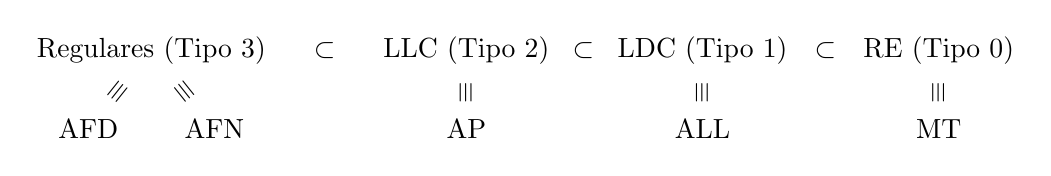
\begin{tikzpicture}[node distance=3cm, every node/.style={sloped}]
  \node (Reg) {Regulares (Tipo 3)};
  \node (LLC) at (4, 0) {LLC (Tipo 2)};
  \node (LDC) at (7, 0) {LDC (Tipo 1)};
  \node (RE) at (10, 0) {RE (Tipo 0)};
  \node (AFD) at (-0.8, -1) {AFD};
  \node (AFN) at (0.8, -1) {AFN};
  \node (AP) at (4, -1) {AP};
  \node (ALL) at (7, -1) {ALL};
  \node (MT) at (10, -1) {MT};
  \path (Reg) -- (LLC) node[midway] {$\subset$};
  \path (LLC) -- (LDC) node[midway] {$\subset$};
  \path (LDC) -- (RE) node[midway] {$\subset$};
  \path (AFD) -- (Reg) node[midway] {$\equiv$};
  \path (AFN) -- (Reg) node[midway] {$\equiv$};
  \path (AP) -- (LLC) node[midway] {$\equiv$};
  \path (ALL) -- (LDC) node[midway] {$\equiv$};
  \path (MT) -- (RE) node[midway] {$\equiv$};
\end{tikzpicture}


\section{O Problema da Parada}
\label{sec:problema-parada}

As diversas variantes de Máquinas de Turing (multifitas, RAM e mesmo as não-determinísticas) são equivalentes a MTs simples.
Além disso vimos que todas as Línguagens Livres de Contexto são recursivas (Teorema \ref{}), ou seja, toda LLC podem ser reconhecidas por uma MT.
Vimos também linguagens que não são livres de contexto e são reconhecidas por MTs.
Assim, parece que chegamos em um modelo que é mais expressivo do que os que vimos até aqui e parece que chegamos em uma espécie de limite -- todas as tentativas de tornar o modelo mais expressivo falharam.
Nesta seção veremos que mesmo esse modelo super-expressivo tem limitações.

Para tanto precisamos fazer uma digressão sobre o conceito de infinito

\subsection*{O infinito de Cantor}

Dizemos que dois conjuntos $A$ e $B$ tem a mesma {\em cardinalidade} se existe uma bijeção entre eles.
Ou seja, se existe alguma função $f: A \to B$ que leva cada elemento de $A$ em um elemento distinto de $B$ ({\em injetora}) de forma que não sobre elementos em $B$ ({\em sobrejetora}).

% aqui deveria vir um diagrama

Note que se $A$ e $B$ são finitos, nossa definição garante que eles possuem a mesma quantidade de elementos (se $A$ possui mais elementos não há como a função $f$ ser injetora e se $B$ possui mais elementos ela não pode ser sobrejetora).
A cardinalidade representa a forma mais primitiva de contagem: uma pedra (do conjunto $A$ das pedras) para cada carneiro (do conjunto $B$ de carneiros).
Quando extrapolamos essa definição para os conjuntos infinitos, temos alguns resultados um pouco contra-intuitivos.

\begin{example}
  O conjunto dos naturais $\mathbb{N}$ tem a mesma cardinalidade do conjunto dos números pares.
  
  Para mostrar isso, basta achar uma função bijetora que leve naturais em pares.
  A função $f(n) = 2n$ faz isso.
\end{example}

O exemplo anterior mostra dois conjuntos infinitos que tem a mesma cardinalidade (mesma quantidade de elementos por assim dizer).
Poderíamos levantar a hipótese de que todo conjunto infinito possui a mesma cardinalidade, mas o teorema a seguir provado por Cantor no final do século XIX mostra que esse não é o caso.

\begin{theorem}[Cantor]
  Seja $A$ um conjunto qualquer, o conjunto $2^A := \{B : B \subseteq A\}$ (chamado conjunto das partes de $A$) tem cardinalidade extritamente maior do que $A$.
\end{theorem}
\begin{proof}
  Suponha por absurdo que exista uma bijeção entre $f: A \to 2^A$ e considere o conjunto $B := \{x \in A : x \notin f(x)\}$.
  Como $B \subseteq A$, por definição $B \in 2^A$.
  Se $f$ fosse bijetora, deveria existir $x \in A$ tal que $f(x) = B$.

  Se $x \in f(x)$, então $x \in B = f(x)$ e nesse caso $x \notin f(x)$ pela definição de $B$, o que seria uma contradição.
  Por outro lado, se $x \notin f(x) = B$ então, pela defição de $B$, temos que $x \in f(x)$, o que também seria uma contradição.

  Concluímos que não existe uma função bijetora entre $A$ e $2^A$.
\end{proof}

Voltemos agora às MTs.
Podemos representar uma MT é descrita como uma sequência de instruções com o seguinte formato:

\begin{displaymath}
  q_0 a \to q_1 b D
\end{displaymath}

Ou seja, podemos representar uma sequência de instruçõe como uma string sobre o alfabeto $\Sigma_{MT} = Q \cup \Sigma \cap \{E, D, \to, \#\}$ (o símbolo $\#$ é usado para separar as instruções).
Existem infinitas MTs, ou equivalentemente, infinitas strings em $\Sigma_{MT}^*$.
Pelo teorema de Cantor vimos que o conjunto $2^{\Sigma_{MT}^*}$ tem cardinalidade maior do que $\Sigma_{MT}^*$.
Ou seja, existem mais linguagens do que MTs.
Concluímos que deve haver linguagens que não são reconhecidas por Máquinas de Turing.
Antes de mostrar um exemplo disso, vamos explorar uma consquência importante do fato de que qualquer MT pode ser descrita como uma string.

\subsection*{Máquina de Turing Universal}

Uma MT universal $U$ recebe $\langle M \rangle \in \Sigma_{MT}^*$ -- a representação de uma MT $M$ -- e uma entrada $x$.
A máquina $U$ e aceita essa entrada se $M$ aceita $x$ e rejeita a entrada se $M$ rejeita $x$\footnote{Para uma descrição compreensível da construção de uma MT universal tal qual descrita por Turing, veja \url{https://plato.stanford.edu/entries/turing-machine/\#TuriUnivMach} (Consultado em outubro de 2020)}.
Em outras palavras $U$ reconhece a seguinte linguagem:

\begin{displaymath}
A_{MT} := \{\langle M, x \rangle  : M \textrm{ aceita } x\} 
\end{displaymath}

A existência de uma MT universal nos mostra que se codificarmos uma única MT, a saber uma MT universal, em um harware, podemos {\em simular} qualquer MT como um software.
Essa descoberta do começo dos anos 30 dá origem ao que hoje chamamos de {\em computação}.


\subsection*{O Problema da Parada}

Note que não dicemos que $U$ decide $A_{MT}$.
Se $M$ aceita $x$, então, por definição $U$ aceita $\langle M, x\rangle$, mas não estabelecemos o que ocorre se $M$ não aceita $x$.
Neste caso, a máquina $U$ não pode aceitar a entrada $\langle M, x \rangle$.
Ela pode rejeitar $\langle M, x \rangle$, mas podem ocorrer outras coisas.
$U$ pode, por exemplo, entrar em loop infinito.
O teorema a seguir mostra que não é possível construir uma MT que decida para a entrada $\langle M, x \rangle$ se a MT $M$ reconhece $x$:

\begin{theorem}
  \label{teo:parada}
  $A_{MT}$ não é recursiva.
\end{theorem}
\begin{proof}
  Suponha por absurdo $A_{MT}$ seja recursiva.
  Por definição, deve existir uma MT $H$ tal que:
  \begin{displaymath}
    H(\langle M, x \rangle) = \left\{\begin{array}{cl}
                 \textrm{aceita} & \textrm{se $M$ aceita $x$}\\
                 \textrm{rejeita} & \textrm{se $M$ não aceita $x$}\\ 
               \end{array}\right.
  \end{displaymath}
  Se essa MT existisse, poderíamos trivialmente construir uma MT $D$ que faz o seguinte:
  \begin{displaymath}
    D(\langle M \rangle) =  \left\{\begin{array}{cl}
                \textrm{aceita} & \textrm{se $M$ não aceita $\langle M \rangle$}\\
                \textrm{rejeita} & \textrm{se $M$ aceita $\langle M \rangle$}\\ 
              \end{array}\right.
  \end{displaymath}

  Temos então que:

  \begin{displaymath}
    D(\langle D \rangle) = \left\{\begin{array}{cl}
               \textrm{aceita} & \textrm{se $D$ não aceita $\langle D \rangle$}\\
               \textrm{rejeita} & \textrm{se $D$ aceita $\langle D \rangle$}\\
             \end{array}\right.
  \end{displaymath}

  Contrariando a definição de $D$.
  Logo, não podem existir uma MT $D$ e, portanto, não pode existir $H$ que decide $A_{MT}$.
\end{proof}

A prova do teorema acima segue uma lógica similar a demonstração do Teorema de Cantor.
Ambas utilizam uma técnica chamada de ``diagonalização''.

\begin{corollary}
  $\overline{A_{MT}}$ não é recursivamente enumerável.
\end{corollary}

$A_{MT}$ é um exemplo de linguagem recursivamente enumerável que não é recursiva.

\subsection*{Tese de Church-Turing}

Nas seções anteriores vimos o quão expressivas são as MTs.
Nesta vimos algumas limitações.

A pergunta que resta é se existe algum modelo de computação mais expressivo do que as Máquinas de Turing.
Ou seja, algum modelo que reconhece um conjunto ainda maior de linguagens.

Nos anos 30 o matemático Alonzo Church levantou a hipótese de que não.
A {\em Tese de Church-Turing}, como ficou conhecida, estabelece que não existem modelos de computação mais expressivos do que as MTs.
Temos três motivos para crer que a hipótese seja válida:
\begin{enumerate}
\item a equivalência entre muitos modelos distintos (não só os que vimos em aqui, mas principalmente as funções recursivas e o cálcula lambda)
\item a existência de uma MT universal
\item a propria simplicidade e generalidade do modelo de Turing
\end{enumerate}

Podemos manter, porém, uma postura cética e aceitar a tese enquanto não se apresenta nenhum outro modelo mais expressivo.

\section{Redutibilidade}
\label{sec:redutibilidade}

Na seção anterior vimos um exemplo de problema indecidível.
Para provar que outros problemas também são indecidíveis usaremos uma técnica chamada redução.
Uma {\em redução} é uma maneira de converter um problema em outro.
Assim se sabemos como resolver um problema $A$ podemos resolver outros problemas reduzindo-os a ele.
Conversamente se sabemos que $A$ não pode ser resolvido e reduzimos $A$ a outro problema $B$ então descobrimos que $B$ também não pode ser resolvido.

\begin{example}
  \label{ex:vazio}
  Considere a linguagem $V_{MT}$ das representações de Máquinas de Turing que reconhecem a linguagem vazia, ou seja, que não reconhecem nenhuma string.

  \begin{displaymath}
    V_{MT} := \{\langle M \rangle : L(M) = \emptyset \} 
  \end{displaymath}

  Vamos reduzir o problema $A_{MT}$ a esse problema.
  Considere as seguintes MTs:

  \begin{displaymath}
    O_{\omega}(x) = \left\{\begin{array}{cl}
                 \textrm{rejeita} & \textrm{se $x \neq \omega$}\\
                 \textrm{aceita} & \textrm{se $M$ aceita $\omega$}\\ 
               \end{array}\right.
  \end{displaymath}

  Note que a máquina $O_\omega$ simula a máquina $M$.
  Além disso, já vimos no Exemplo \ref{ex:eq} que é possível construir uma MT que verifica se duas strings são iguais.

  Agora suponha por absurdo que exista uma MT $R$ que decide $V_{MT}$.
  Poderíamos, portanto, construir a seguinta máquina:

  \begin{displaymath}
    S(\langle M, \omega \rangle) = \left\{\begin{array}{cl}
                 \textrm{rejeita} & \textrm{se $R$ aceita $\langle O_\omega \rangle$}\\
                 \textrm{aceita} & \textrm{se $R$ rejeita $\langle O_\omega \rangle$}\\ 
               \end{array}\right.
  \end{displaymath}

  Se $R$ aceita $\langle O_\omega \rangle$ então $L(O_\omega) = \emptyset$ e, portanto, $M$ não aceita $\omega$ (caso contrário $\omega \in L(O_\omega)$).
  Ou seja, se $S$ rejeita $\langle M, \omega \rangle$ então $M$ não aceita $\omega$.

  Por outro lado, se $R$ rejeita $\langle O_\omega \rangle$ então $L(O_\omega) \neq \emptyset$ e, portanto, $M$ aceita $\omega$.
  Ou seja, se $S$ aceita $\langle M, \omega \rangle$ se e somente se $M$ aceita $\omega$.

  Em outras palavras $L(S) = A_{MT}$.

  Pelo Teorema \ref{teo:parada} sabemos que $A_{MT}$ é indecidível.
  Portanto, $S$ não pode existir.
  Vimos, porém, que a existência de $R$ implica que somos capazes de construir $S$.
  Concluímos que $R$, uma máquina que decide $V_{MT}$, não pode existir.
  Ou seja, $V_{MT}$ é indecidível.
\end{example}

Existem várias maneiras de definir formalmente o conceito de {\em redução} de um problema $A$ para um problema $B$.
Focaremos em um tipo.
A {\em redução por mapeamento} determina que existe uma {\em função computável} $f$ que converte instâncias do problema $A$ em instâncias de $B$.

\begin{definition}{Função Computável}
  Uma função $f: \Sigma^* \to \Sigma^*$ é {\em computável} se existe alguma MT $M$ que para toda entrada $\omega$ pára exatamente com $f(\omega)$ na fita.
\end{definition}

\begin{definition}{Redução por mapeamento}
  A linguagem $A$ é {\em redutível por mapeamento} à linguagem $B$ (escrevemos $A \leq_m B$) se existe um função computável $f : \Sigma^* \to \Sigma^*$ tal que:
  \begin{displaymath}
    \omega \in A \textrm{ se e somente se } f(\omega) \in B
  \end{displaymath}
\end{definition}

Derivamos dois resultados diretos dessa definição:

\begin{corollary}
  Se $A \leq_m B$ e $B$ é decidível, então $A$ é decidível.
\end{corollary}
\begin{proof}
  Se $B$ é decidível então existe uma MT $M_B$ que decide $B$ -- ou seja, que aceita todas as strings $\omega \in B$ e rejeita todas as strings $\omega \notin B$.
  Como $A \leq_m B$, por definição, existe $f$ computável que reduz de $A$ para $B$.
  Podemos então construir uma MT $M_A$ que decide $A$ da seguinte forma:

 \begin{displaymath}
    M_A(\omega) = \left\{\begin{array}{cl}
                 \textrm{aceita} & \textrm{se $M_B$ aceita $f(\omega)$}\\
                 \textrm{rejeita} & \textrm{se $M_B$ rejeita $f(\omega)$}\\ 
               \end{array}\right.
  \end{displaymath}  
\end{proof}

\begin{corollary}
  Se $A \leq_m B$ e $A$ é indecidível, então $B$ é indecidível.
\end{corollary}

\begin{example}
  Vamos usar a redução por mapeamento para mostrar que a seguinte linguagem é indecidível:
  \begin{displaymath}
    EQ_{MT} := \{\langle M_1, M_2 \rangle : L(M_1) = L(M_2)\}
  \end{displaymath}

  Considere a função $f$ que recebe como entrada $\langle M \rangle$ e produz como saída $\langle M, M_\bot\rangle$ em que $M_\bot$ é uma MT que rejeita qualquer entrada.
  É faćil notar que $f$ é computável, basta criar uma MT que concatena na entrada a descrição da MT $M_\bot$, que é fácil de construir.
  Essa função reduz o problema $V_{MT}$ ao problema $EQ_{MT}$, portanto, $V_{MT} \leq_m EQ_{MT}$.
  No Exemplo \ref{ex:vazio} vimos que $V_{MT}$ não é decidível e concluímos que $EQ_{MT}$ também não é.
\end{example}

Vimos até aqui três problemas indecidíveis -- $A_{MT}$, $V_{MT}$ e $EQ_{MT}$.
Os três recebem como entrada a codificação de uma ou mais MTs.
Para concluir o capítulo vamos apresentar um exemplo de problema indecidível que recebe outro tipo de entrada.
O problema a seguir foi concebido por Emil Post um cientista russo contemporâneo ao Turing que concebeu um modelo de computação muito similar ao que vimos neste capítulo.
A prova da indecidibilidade desse problema é uma redução de $A_{MT}$ a ele, mas será omitida por conter muitos detalhes técnicos pouco interessantes.

\begin{example}
  Considere um conjunto de pares de strings $\{\langle t_1, b_1 \rangle, \langle t_2, b_2 \rangle, \dots, \langle t_k, b_k \rangle\}$ em que $t_i, b_i \in \Sigma^*$.
  Um {\em emparelhamento} é uma sequência desses pares de strings de forma que a concatenação dos $t$s seja idêntica a concatenação dos $b$s.
  (Note que não exigimos que cada par $\langle t, b \rangle$ ocorra uma única vez.)

  Se preferirem, podemos imaginar um par $\langle t, b \rangle$ como uma espécie de pedra de dominó.
  No exemplo a seguir temos um emparelhamento válido com o alfabeto $\Sigma = \{a,b,c\}$.
  A entrada é dada pelo seguinte conjunto:

  \begin{displaymath}
    \Big\{  \left[\frac{ca}{a}\right], \left[\frac{b}{ca}\right], \left[\frac{abc}{c}\right], \left[\frac{a}{ab}\right] \Big\}
  \end{displaymath}

  O seguinte é um emparelhamento válido:

  \begin{displaymath}
    \left[\frac{a}{ab}\right] \left[\frac{b}{ca}\right] \left[\frac{ca}{a}\right] \left[\frac{a}{ab}\right] \left[\frac{abc}{c}\right]
  \end{displaymath}

  Esse emparelhamento é válido pois a concatenação das strings da parte de cima do dominó coincide com a concatenação de baixo:
  \begin{displaymath}
    abcaaabc
  \end{displaymath}
  
  O {\em Problema da Correspondência de Post} (PCP) é o seguinte.
  Dado um conjunto de pares de strings (peças de dominó), determinar se existe um emparelhamento válido para esse conjunto.
  Esse problema pode ser descrito por meio da seguinte linguagem:
  
  \begin{displaymath}
    PCP := \{\langle P \rangle : P \textrm{ é uma instância que possui emparelhamento }\}
  \end{displaymath}

  Como adiantamos, a linguagem PCP é indecidível.
\end{example}

